% Begin the document and set up the style of the document
\documentclass[a4paper]{article}

% Install the required packages for the document 
\usepackage{envmath}
\usepackage{esvect}
\usepackage{graphicx}
\usepackage{gensymb}
\usepackage{tikz}
\usepackage[mathcal]{euscript}
\usepackage{geometry}
\usepackage{enumitem}
\usepackage{mathtools}
\usepackage{graphicx}
\usepackage{amsmath}
\usepackage{amscd}
\usepackage{amssymb}
\usepackage{amsfonts}
\usepackage{harpoon}
\usepackage{pgf}
\usepackage{tikz}
\usepackage{mathrsfs}
\usepackage{asyalign}
\usepackage{physics}
\usepackage{enumitem}
\usepackage{xhfill}
\usepackage{accents}
\usepackage{cite}
\usepackage{url}
\usepackage[tableposition=top]{caption}
\usepackage{ifthen}
\usepackage[utf8]{inputenc}
\usepackage{tikz-3dplot}
\usetikzlibrary{patterns}
\usetikzlibrary{arrows}

% Page and style settings
\parskip=8pt
\parindent=0pt
% Right margin
\textwidth=6.25in
% Left margin
\oddsidemargin=0pt
\evensidemargin=0pt
% Bottom margin
\textheight=10in
% Top margin
\topmargin=-0.75in
\baselineskip=11pt
% end of page and other style settings

\renewcommand{\familydefault}{\sfdefault}


% Begin the text of the document
\begin{document}

% Begin the Title Page
\begin{titlepage}

\newcommand{\HRule}{\rule{\linewidth}{0.5mm}} % Defines a new command for the horizontal lines, change thickness here

\center % Center everything on the page
 
\textsc{\LARGE University of Sydney}\\[1.5cm] % Name of your university/college
\textsc{\Large MATH 1907}\\[0.5cm] % Major heading such as course name
\textsc{\large SSP}\\[0.5cm] % Minor heading such as course title

\HRule \\[0.4cm]
{ \huge \bfseries Assignment 2 - Euler's Formula}\\[0.4cm] % Title of your document
\HRule \\[1.5cm]

\begin{minipage}{0.4\textwidth}
\begin{flushleft} \large
\emph{Author:}
Keegan Gyoery % Your name
\\
\emph{SID:}
470413467
\end{flushleft}
\end{minipage}
~
\begin{minipage}{0.4\textwidth}
\begin{flushright} \large
\emph{Lecturer:} 
Oded Yacobi % Tutor's Name
\\
\emph{Seminar:}
New Law Annexe SR 346
Tuesday 4pm
\end{flushright}
\end{minipage}\\[4cm]

{\large October 5, 2017}\\[3cm] % Date, change the \today to a set date if you want to be precise

\vfill % Fill the rest of the page with whitespace

\end{titlepage}

\pagenumbering{arabic}

\begin{enumerate}[label=\textbf{\arabic*.}]
	\item 
	\begin{enumerate}
		\item Let $\displaystyle{G}$ be the graph below. We are required to prove for the graph $\displaystyle{G}$, that any cycle must have length at least 4.

		\bigbreak

		\begin{center}
			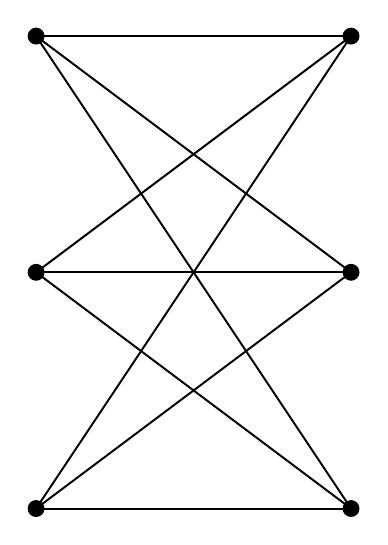
\begin{tikzpicture}

				\draw[line width = 0.25mm] (-2,-3) -- (2,3);
				\draw[line width = 0.25mm] (-2,3) -- (2,-3);
				\draw[line width = 0.25mm] (-2,3) -- (2,3);
				\draw[line width = 0.25mm] (-2,-3) -- (2,-3);
				\draw[line width = 0.25mm] (-2,0) -- (2,0);
				\draw[line width = 0.25mm] (-2,-3) -- (2,0);
				\draw[line width = 0.25mm] (-2,3) -- (2,0);
				\draw[line width = 0.25mm] (2,3) -- (-2,0);
				\draw[line width = 0.25mm] (2,-3) -- (-2,0);
				\draw[fill] (-2,3) circle (1mm);
				\draw[fill] (2,3) circle (1mm);
				\draw[fill] (-2,0) circle (1mm);
				\draw[fill] (2,0) circle (1mm);
				\draw[fill] (-2,-3) circle (1mm);
				\draw[fill] (2,-3) circle (1mm);

			\end{tikzpicture}
		\end{center}

		\bigbreak

		In order to prove the result that $\displaystyle{G}$ has cycle length of at least 4, we must first prove that $\displaystyle{G}$ has two vertex sets. In order to prove this, we must first define what is meant by a vertex set. A vertex set is the set of vertices that are not connected to any other vertex in the set. Vertices then can only be connected with a vertex from another vertex set. Thus, an elegant way to determine the number of vertex sets a graph has is to colour the vertices from the same set a single, distinct colour.

		\bigbreak

		Using the following diagram, we can see that $\displaystyle{G}$ can be coloured using two colours.

		\bigbreak

		\begin{center}
			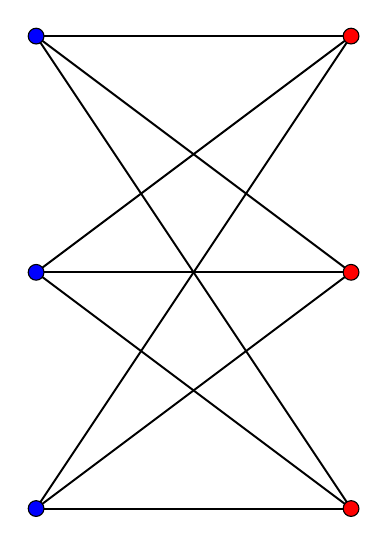
\begin{tikzpicture}

				\draw[line width = 0.25mm] (-2,-3) -- (2,3);
				\draw[line width = 0.25mm] (-2,3) -- (2,-3);
				\draw[line width = 0.25mm] (-2,3) -- (2,3);
				\draw[line width = 0.25mm] (-2,-3) -- (2,-3);
				\draw[line width = 0.25mm] (-2,0) -- (2,0);
				\draw[line width = 0.25mm] (-2,-3) -- (2,0);
				\draw[line width = 0.25mm] (-2,3) -- (2,0);
				\draw[line width = 0.25mm] (2,3) -- (-2,0);
				\draw[line width = 0.25mm] (2,-3) -- (-2,0);
				\draw[fill = blue] (-2,3) circle (1mm);
				\draw[fill = red] (2,3) circle (1mm);
				\draw[fill = blue] (-2,0) circle (1mm);
				\draw[fill = red] (2,0) circle (1mm);
				\draw[fill = blue] (-2,-3) circle (1mm);
				\draw[fill = red] (2,-3) circle (1mm);

			\end{tikzpicture}
		\end{center}

		\bigbreak

		As a result, $\displaystyle{G}$ has two vertex sets. Next, we need to examine the cycle lengths of the graph $\displaystyle{G}$. The graph $\displaystyle{G}$ cannot have any cycles of length 1, by definition of a cycle. Furthermore, $\displaystyle{G}$ has no parallel edges, and thus cannot have a cycle of length 2. Finally, as we proved that $\displaystyle{G}$ has only two vertex sets, there can be no cycles of length 3. This result arises from the definition that a cycle of length 3 requires at least three vertex sets. With two vertex sets, $\displaystyle{G}$ cannot have a cycle of length 3. Thus, all cycles in $\displaystyle{G}$ must have length 4 or greater.

		\pagebreak

		\item We are now required to prove that the graph $\displaystyle{G}$ is not planar, using Euler's Formula. In order to do so, we will use the definition of a bipartite graph, and Euler's Formula. Euler's Formula is as follows.
		\begin{align*}
		n - e + f & = 2\\
		\end{align*}
		Euler's Formula holds for all planar graphs. Moreover, by the definition of a bipartite graph, $\displaystyle{G}$ has two independent vertex sets, meaning that no vertex is connected to another vertex from the same set. Thus, in the graph of $\displaystyle{G}$, no red vertex is connected to another red vertex, and the same result holds for the blue vertices. We will now assume that $\displaystyle{G}$ has a triangular face, that is a face enclosed by 3 edges. In order for this to be true, a vertex must connect with a vertex from its own vertex set, to form a triangular face with 3 edges. However, due to the nature of $\displaystyle{G}$ as a bipartite graph, no vertex can connect to another vertex in its own set. Thus, $\displaystyle{G}$ cannot have any triangular faces, which are made up of 3 edges. As a result, all faces must be enclosed by 4 or more edges. 

		\bigbreak

		Using the result above, and the graph of $\displaystyle{G}$, we next assume that $\displaystyle{G}$ is planar. Thus, Euler's Formula holds. From the graph, we have the following results.
		\begin{align*}
		n & = 6\\
		e & = 9\\
		\therefore 2 & = n - e + f\\
		\therefore f & = 2 + e - n\\
		& = 2 + 9 - 6\\
		\therefore f & = 5\\ 
		\end{align*}
		Thus, if $\displaystyle{G}$ is a planar graph it must have 5 faces. Now, as each face in the graph of $\displaystyle{G}$ must be enclosed by at least 4 edges, then in the minimum case scenario, there must be 20 edges, as each of the 5 faces requires 4 edges. However, this is double counting edges, as each edge is in fact shared by two faces. Thus again, in the minimum case scenario, the number of edges required for the graph of $\displaystyle{G}$ is 10. This clearly contradicts the actual graph of $\displaystyle{G}$ which obviously has 9 edges. Thus, by contradiction, $\displaystyle{G}$ cannot be a planar graph.

	\end{enumerate}

	\bigbreak

	\item We are now required to prove that for $\displaystyle{G}$, a simple plane graph with $\displaystyle{n>2}$ vertices, that $\displaystyle{G}$ has at most $\displaystyle{3n-6}$ edges. By the definition of simple, $\displaystyle{G}$ has no loops or parallel edges. As $\displaystyle{G}$ is planar, we can add edges to make every face into a triangle. By making every face a triangle, we have used the maximum number of edges possible for the graph $\displaystyle{G}$. Let $\displaystyle{G}$ have $\displaystyle{f}$ faces, $\displaystyle{e}$ edges, and $\displaystyle{n}$ vertices. Now, with double counting the number of edges in the graph, we have $\displaystyle{3f}$ edges, as each face is triangular and thus surrounded by 3 edges. However, each edge is shared by two faces, thus, we have double counted by a factor of 2. As a consequence, we get the following result.
	\begin{align*}
	3f & = 2e\\
	\therefore f & = \frac{2}{3}e\\
	\end{align*} 
	Now, using Euler's Formula, we have the following result.
	\begin{align*}
	n - e + f & = 2\\
	n - e + \frac{2}{3}e & = 2\\
	n - \frac{1}{3}e & = 2\\
	\therefore 3n - e & = 6\\
	\therefore e & = 3n - 6\\
	\end{align*}
	As the scenario where every face is triangular uses the maximum amount of edges possible for the graph $\displaystyle{G}$, the graph $\displaystyle{G}$ then has at most $\displaystyle{3n-6}$ edges.

	\pagebreak

	\item
	\begin{enumerate} 
		\item The Euler characteristic of any polyhedron is computed by the following formula, using $\displaystyle{E_{c}}$ to denote the Euler characteristic.
		\begin{align*}
		E_{c} & = n - e + f\\
		\end{align*} 
		In the given polyhedron, a torus, we have the following results.
		\begin{align*}
		n & = 16\\
		e & = 32\\
		f & = 16\\
		\therefore E_{c} & = n - e + f\\
		& = 16 - 32 + 16\\
		\therefore E_{c} & = 0\\
		\end{align*}
		Thus it is clear that the Euler characteristic of the given polyhedron, a torus, is 0.

		\bigbreak

		\item We are now asked to compute the Euler characteristic of a torus with two shafts removed. The diagram of the simplest scenario is given below.

		\bigbreak

		\begin{center}

		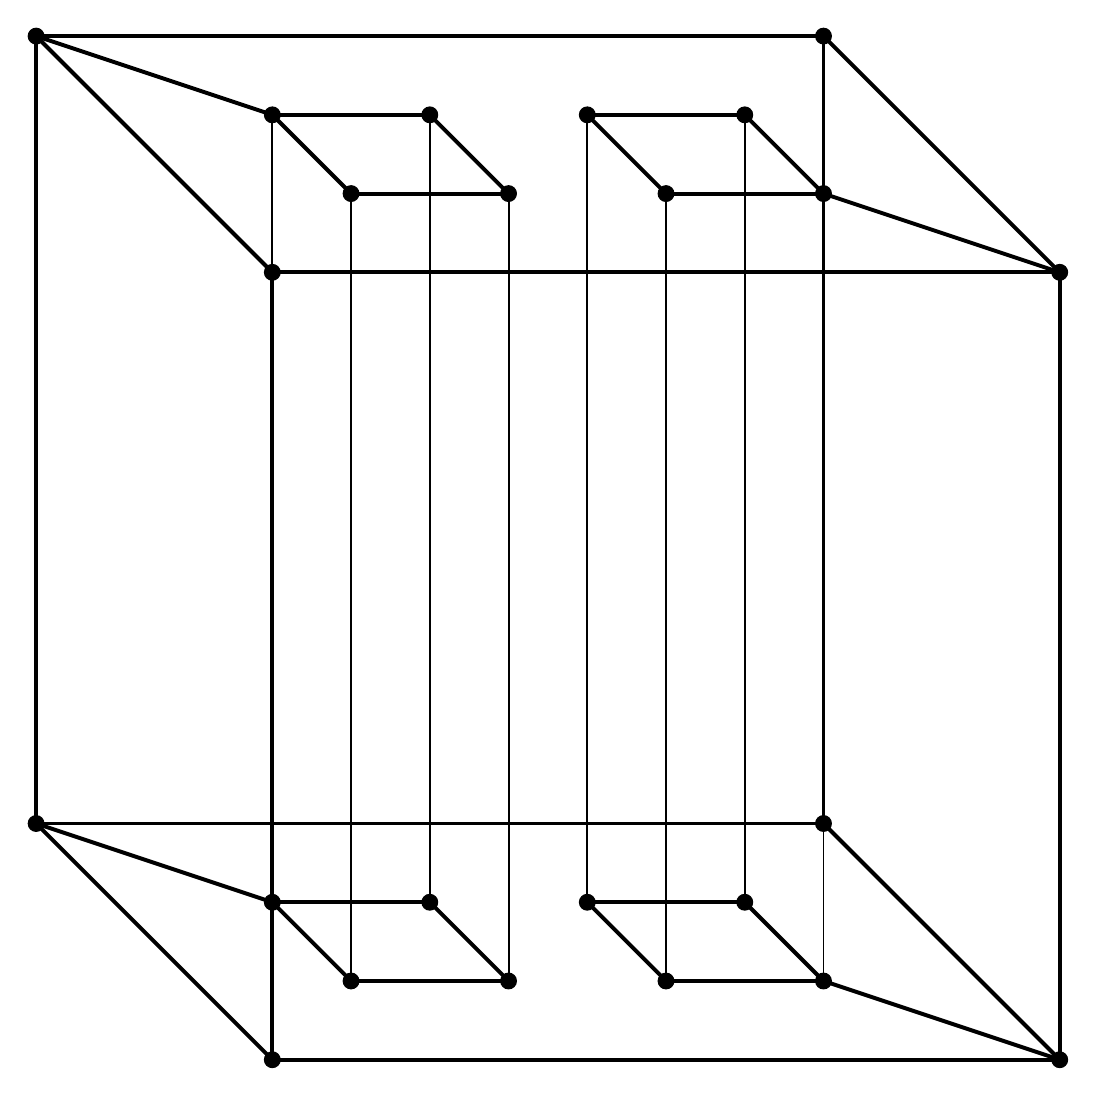
\begin{tikzpicture}

			\draw[line width = 0.5mm] (-3,3) -- (7,3);
			\draw[line width = 0.5mm] (0,0) -- (10,0);
			\draw[line width = 0.5mm] (-3,3) -- (0,0);
			\draw[line width = 0.5mm] (7,3) -- (10,0);
			\draw[line width = 0.5mm] (-3,3) -- (-3,-7);
			\draw[line width = 0.5mm] (0,0) -- (0,-10);
			\draw[line width = 0.5mm] (10,0) -- (10,-10);
			\draw[line width = 0.5mm] (7,3) -- (7,-7);
			\draw[line width = 0.5mm] (-3,-7) -- (7,-7);
			\draw[line width = 0.5mm] (-3,-7) -- (0,-10);
			\draw[line width = 0.5mm] (0,-10) -- (10,-10);
			\draw[line width = 0.5mm] (7,-7) -- (10,-10);

			\draw[line width = 0.5mm] (0,2) -- (2,2);
			\draw[line width = 0.5mm] (0,2) -- (1,1);
			\draw[line width = 0.5mm] (1,1) -- (3,1);
			\draw[line width = 0.5mm] (2,2) -- (3,1);
			\draw[line width = 0.25mm] (0,2) -- (0,-8);
			\draw[line width = 0.25mm] (2,2) -- (2,-8);
			\draw[line width = 0.25mm] (1,1) -- (1,-9);
			\draw[line width = 0.25mm] (3,1) -- (3,-9);
			\draw[line width = 0.5mm] (1,-9) -- (0,-8);
			\draw[line width = 0.5mm] (0,-8) -- (2,-8);
			\draw[line width = 0.5mm] (3,-9) -- (1,-9);
			\draw[line width = 0.5mm] (2,-8) -- (3,-9);

			\draw[line width = 0.5mm] (4,2) -- (6,2);
			\draw[line width = 0.5mm] (4,2) -- (5,1);
			\draw[line width = 0.5mm] (5,1) -- (7,1);
			\draw[line width = 0.5mm] (6,2) -- (7,1);
			\draw[line width = 0.25mm] (4,2) -- (4,-8);
			\draw[line width = 0.25mm] (6,2) -- (6,-8);
			\draw[line width = 0.25mm] (5,1) -- (5,-9);
			\draw[line width = 0.25mm] (7,1) -- (7,-9);
			\draw[line width = 0.5mm] (5,-9) -- (4,-8);
			\draw[line width = 0.5mm] (4,-8) -- (6,-8);
			\draw[line width = 0.5mm] (7,-9) -- (5,-9);
			\draw[line width = 0.5mm] (6,-8) -- (7,-9);

			\draw[line width = 0.5mm] (-3,3) -- (0,2);
			\draw[line width = 0.5mm] (10,0) -- (7,1);
			\draw[line width = 0.5mm] (-3,-7) -- (0,-8);
			\draw[line width = 0.5mm] (10,-10) -- (7,-9);

			\draw[fill] (-3,3) circle (1mm);
			\draw[fill] (7,3) circle (1mm);
			\draw[fill] (0,0) circle (1mm);
			\draw[fill] (10,0) circle (1mm);
			\draw[fill] (-3,-7) circle (1mm);
			\draw[fill] (0,-10) circle (1mm);
			\draw[fill] (10,-10) circle (1mm);
			\draw[fill] (7,-7) circle (1mm);
			\draw[fill] (0,2) circle (1mm);
			\draw[fill] (2,2) circle (1mm);
			\draw[fill] (1,1) circle (1mm);
			\draw[fill] (3,1) circle (1mm);
			\draw[fill] (4,2) circle (1mm);
			\draw[fill] (6,2) circle (1mm);
			\draw[fill] (5,1) circle (1mm);
			\draw[fill] (7,1) circle (1mm);
			\draw[fill] (0,-8) circle (1mm);
			\draw[fill] (2,-8) circle (1mm);
			\draw[fill] (1,-9) circle (1mm);
			\draw[fill] (3,-9) circle (1mm);
			\draw[fill] (4,-8) circle (1mm);
			\draw[fill] (6,-8) circle (1mm);
			\draw[fill] (5,-9) circle (1mm);
			\draw[fill] (7,-9) circle (1mm);

		\end{tikzpicture}

		\end{center}

		\pagebreak

		In the given polyhedron, we have the following results.
		\begin{align*}
		n & = 24\\
		e & = 40\\
		f & = 14\\
		\therefore E_{c} & = n - e + f\\
		& = 24 - 40 + 14\\
		\therefore E_{c} & = -2\\
		\end{align*}
		Thus it is clear that the Euler characteristic of the given polyhedron is -2.

		\bigbreak

		\item We are now required to conjecture a formula for the Euler characteristic of a similar polyhedron, except with $\displaystyle{g}$ holes, that is $\displaystyle{g}$ shafts removed from the polyhedron. In order to conjecture a formula, we will consider the Euler characteristics of polyhedrons with $\displaystyle{g}$ shafts removed, for small values of $\displaystyle{g}$. The following table summarises the results.

		\begin{center}
		\begin{tabular}{c|c c c c c}
		\text{$\displaystyle{g}$} & 0 & 1 & 2 & 3 & 4 \\
		\hline
		\text{$\displaystyle{E_{c}}$} & 2 & 0 & -2 & -4 & -6 \\
		\end{tabular}
		\end{center}

		As a result, we get the following conjecture for the Euler characteristic of a polyhedron with g shafts removed.
		\begin{align*}
		E_{c} & = -2(g-1)\\
		\therefore E_{c} & = 2(1-g)\\
		\therefore n - e + f & = 2(1-g)\\
		\end{align*}

		\bigbreak

		\item We are now required to prove the conjecture that we provided in part (c), which we will do so using induction. In order to complete the induction proof, we first need to establish some notation and secondly, establish how to describe a hole being added to the polyhedron in terms of faces, edges and vertices.

		\bigbreak

		Firstly, we will define the notation that we are going to use. Foremost, $\displaystyle{E_{c_{k}}}$ is the Euler characteristic of a polyhedron with $\displaystyle{k}$ holes removed. Secondly, $\displaystyle{n_{k}}$, $\displaystyle{e_{k}}$ and $\displaystyle{f_{k}}$ are the vertices, edges and faces of a polyhedron with $\displaystyle{k}$ holes removed. Finally, the notation with the subscript $\displaystyle{add}$ indicates the results of adding a hole to the polyhedron.

		\bigbreak

		Secondly, we must examine what happens when a hole is added to a polyhedron. As there are many different ways to draw the new hole into the polyhedron, they must all be equivalent, that is, have the same Euler characteristic, otherwise we can derive topologically different polyhedra by changing the location of a single valid edge, which clearly makes no sense. As a result, we will consider the simplest case, to make the proof as straightforward as possible. The simplest case that ensures the polyhedron remains connected when the hole is added means that after adding the hole, only two further edges must be added to the top and bottom faces to connect the new edges of the hole to the existing polyhedron. Thus, there remains only one face on the top and bottom of the polyhedron. As a result, adding a hole gives the following results for vertices, edges and faces.
		\begin{align*}
		n_{add} & = 8\\
		e_{add} & = 14\\
		f_{add} & = 4\\
		\therefore E_{c_{add}} & = n_{add} - e_{add} + f_{add}\\
		& = 8 - 14 + 4\\
		\therefore E_{c_{add}} & = -2\\
		\end{align*}

		\pagebreak

		With use of the above results and definitions, we are able to begin the induction to prove the conjecture that for a polyhedron with $\displaystyle{g}$ holes removed, the Euler characteristic is given by 
		\begin{align*}
		E_{c_g} & = 2(1-g)\\
		\end{align*}
		where $\displaystyle{E_{c_g} = n_g - e_g + f_g}$.

		\bigbreak

		The above statement holds for all $\displaystyle{g \in \mathbb{N}}$. For our purposes, the set $\displaystyle{\mathbb{N}}$ includes 0. Thus in order to begin the proof by induction, we first must show that the above result holds for $\displaystyle{g=0}$. 
		\begin{align*}
		E_{c_0} & = 2(1-0)\\
		LHS & = E_{c_0}\\
		& = n_0 - e_0 + f_0\\
		& = 8 - 12 + 6\\
		\therefore LHS & = 2\\
		RHS & = 2(1-0)\\
		\therefore RHS & = 2\\
		\therefore LHS & = RHS\\
		\end{align*}
		Thus the conjecture holds for $\displaystyle{g=0}$. We will now assume that the conjecture holds for $\displaystyle{g=k}$. 
		\begin{align*}
		E_{c_{k}} & = 2(1-k) \dots \dots \dots (*)\\
		\end{align*}
		Now we will consider the conjecture for $\displaystyle{g=k+1}$. 
		\begin{align*}
		E_{c_{k+1}} & = 2\big[1-(k+1)\big]\\
		LHS & = E_{c_{k+1}}\\
		& = n_{k+1} - e_{k+1} + f_{k+1}\\
		& = n_{k} + n_{add} - e_{k} - e_{add} + f_{k} + f_{add}\\
		& = n_{k} - e_{k} + f_{k} + n_{add} - e_{add} + f_{add}\\
		& = E_{c_{k}} + E_{c_{add}}\\
		& = 2(1-k) - 2 \hspace{5mm} \text{by assumption $(*)$}\\
		& = 2 - 2k - 2\\
		& = 2 - 2(k+1)\\
		& = 2\big[1-(k+1)\big]\\
		\therefore LHS & = RHS\\
		\end{align*}
		This completes the induction, and proves the conjecture holds for all values of $\displaystyle{g \in \mathbb{N}}$.

	\end{enumerate}


\end{enumerate}





\end{document}